\section{Практика}
\subsection{Задания}
\begin{itemize}
    \item Определить и обозначить количество узлов, ветвей и контуров. Посчитать и обозначить количество независимых узлов. Посчитать количество необходимых независимых контуров и выбрать независимые контура.
    \item Проанализировать электрическую цепь на предмет наличия параллельных и последовательных соединений, треугольника и звезды. В случае их наличия упростить схему методом эквивалентных преобразований. 
    \item Расставить направления токов в узлах, а также определить направления обхода по независимым контурам
    \item Выбрать независимые узлы и независимые контура для составления уравнений по законам Кирхгофа.
    \item  Составить уравнения по законам Кирхгофа для узлов и контуров.
    \item Составить и упростить систему алгебраических уравнений по законам Кирхгофа.
    \item Составить матрицу A и вектор B и найти X - вектор токов в ветвях.
\end{itemize}


\subsection{Варианты заданий}

\begin{table}[H]
\centering
\caption{Параметры источников и элементов}
\begin{tabular}{|c|c|c|c|c|c|c|c|c|c|}
\hline
\multirow{2}{*}{No} & \multicolumn{3}{c|}{\textbf{Источники}} & \multicolumn{6}{c|}{\textbf{Элементы}} \\
\cline{2-4}\cline{5-10}
& $E_1$, В & $E_2$, В & $J$, А & $R_1$, Ом & $R_2$, Ом & $R_3$, Ом & $R_4$, Ом & $R_5$, Ом & $R_6$, Ом \\
\hline
1 & 40 & 20 & 4 & 5 & 2 & 10 & 5 & 6 & 8 \\
2 & 20 & 40 & 2 & 2 & 1 & 30 & 10 & 10 & 2 \\
3 & 40 & 10 & 6 & 4 & 5 & 3 & 3 & 4 & 2 \\
4 & 10 & 40 & 8 & 6 & 3 & 5 & 5 & 10 & 5 \\
5 & 50 & 20 & 1 & 2 & 1 & 30 & 10 & 10 & 2 \\
\hline
6 & 20 & 50 & 3 & 6 & 8 & 5 & 10 & 9 & 4 \\
7 & 60 & 20 & 7 & 4 & 2 & 6 & 6 & 8 & 5 \\
8 & 20 & 60 & 9 & 3 & 1 & 2 & 8 & 10 & 4 \\
9 & 10 & 30 & 5 & 5 & 4 & 1 & 4 & 5 & 8 \\
10 & 30 & 10 & 10 & 3 & 4 & 10 & 4 & 6 & 3 \\
\hline
11 & 10 & 50 & 4 & 6 & 7 & 8 & 6 & 3 & 5 \\
12 & 50 & 10 & 2 & 7 & 8 & 9 & 10 & 5 & 7 \\
13 & 60 & 10 & 6 & 6 & 7 & 10 & 5 & 3 & 2 \\
14 & 10 & 60 & 8 & 7 & 9 & 6 & 10 & 8 & 6 \\
15 & 10 & 70 & 1 & 6 & 8 & 9 & 5 & 7 & 9 \\
\hline
16 & 70 & 10 & 3 & 8 & 9 & 10 & 7 & 5 & 6 \\
17 & 80 & 20 & 7 & 7 & 8 & 6 & 9 & 5 & 10 \\
18 & 20 & 80 & 9 & 6 & 9 & 10 & 5 & 7 & 8 \\
19 & 80 & 10 & 5 & 7 & 8 & 9 & 10 & 5 & 7 \\
20 & 10 & 80 & 10 & 6 & 7 & 9 & 8 & 10 & 8 \\
\hline
\end{tabular}
\label{tab:parameters}
\end{table}

\subsection{Электрические цепи постоянного тока по заданиям}

% Ряд 1: Задачи 1-2
\begin{figure}[H]
    \centering
    \begin{minipage}{0.48\textwidth}
        \centering
        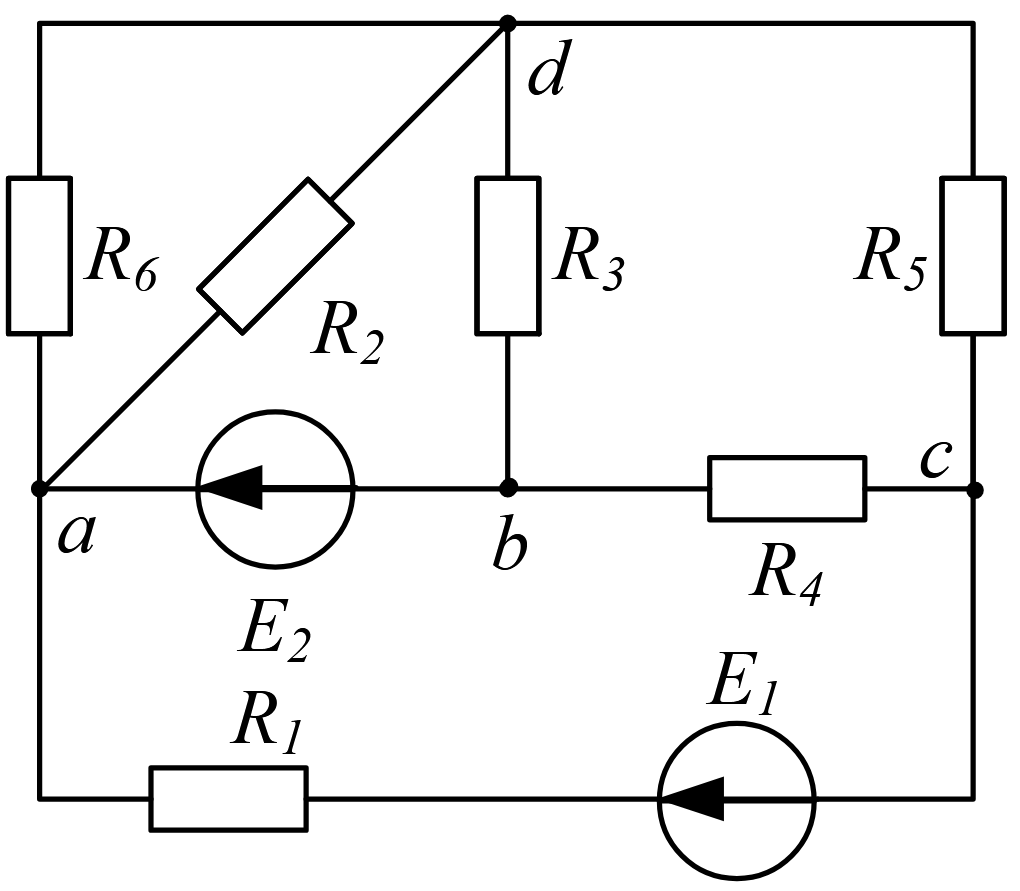
\includegraphics[width=\textwidth]{images/1_task.png}
        \caption{Вариант \#1}
        \label{fig:task_1}
    \end{minipage}
    \hfill
    \begin{minipage}{0.48\textwidth}
        \centering
        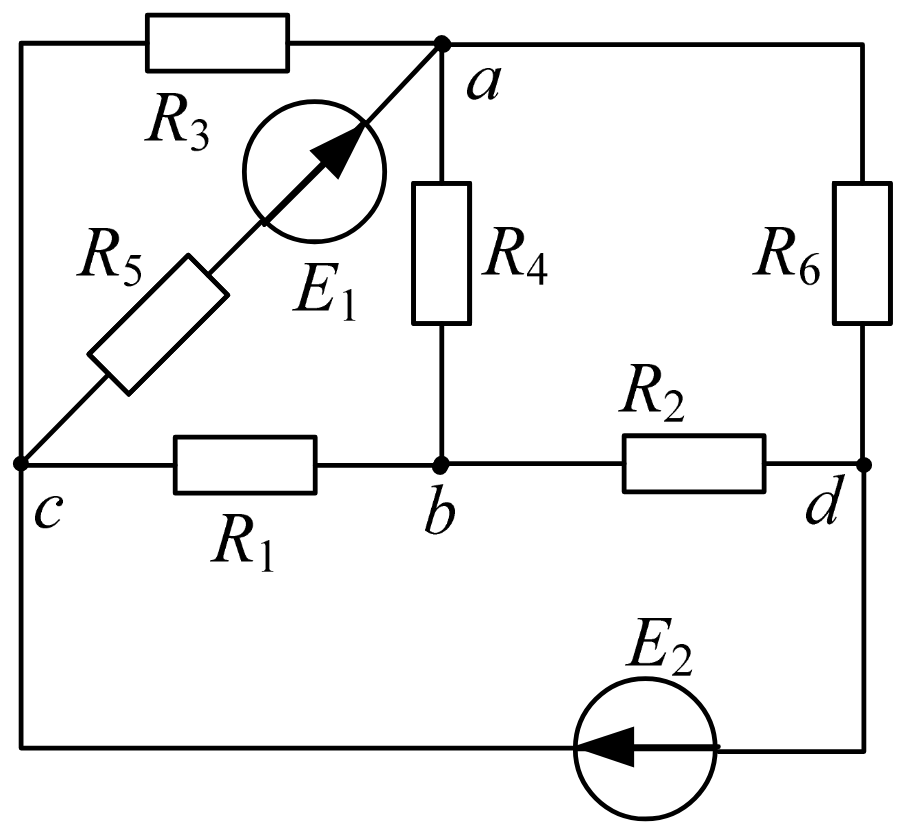
\includegraphics[width=\textwidth]{images/2_task.png}
        \caption{Вариант \#2}
        \label{fig:task_2}
    \end{minipage}
\end{figure}

% Ряд 2: Задачи 3-4
\begin{figure}[H]
    \centering
    \begin{minipage}{0.48\textwidth}
        \centering
        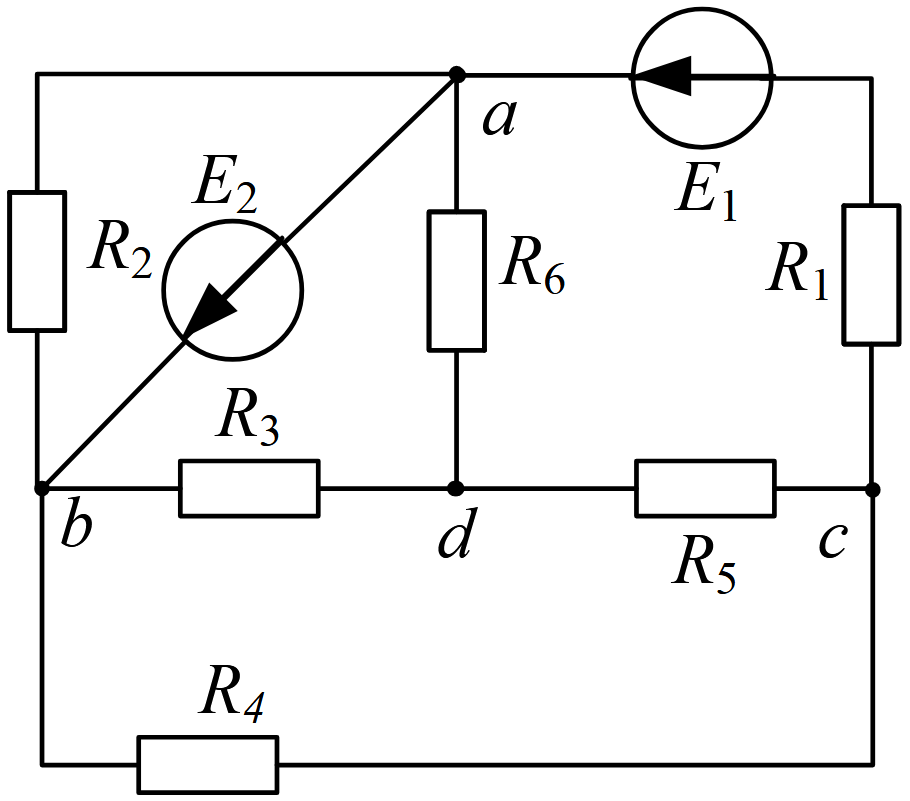
\includegraphics[width=\textwidth]{images/3_task.png}
        \caption{Вариант \#3}
        \label{fig:task_3}
    \end{minipage}
    \hfill
    \begin{minipage}{0.48\textwidth}
        \centering
        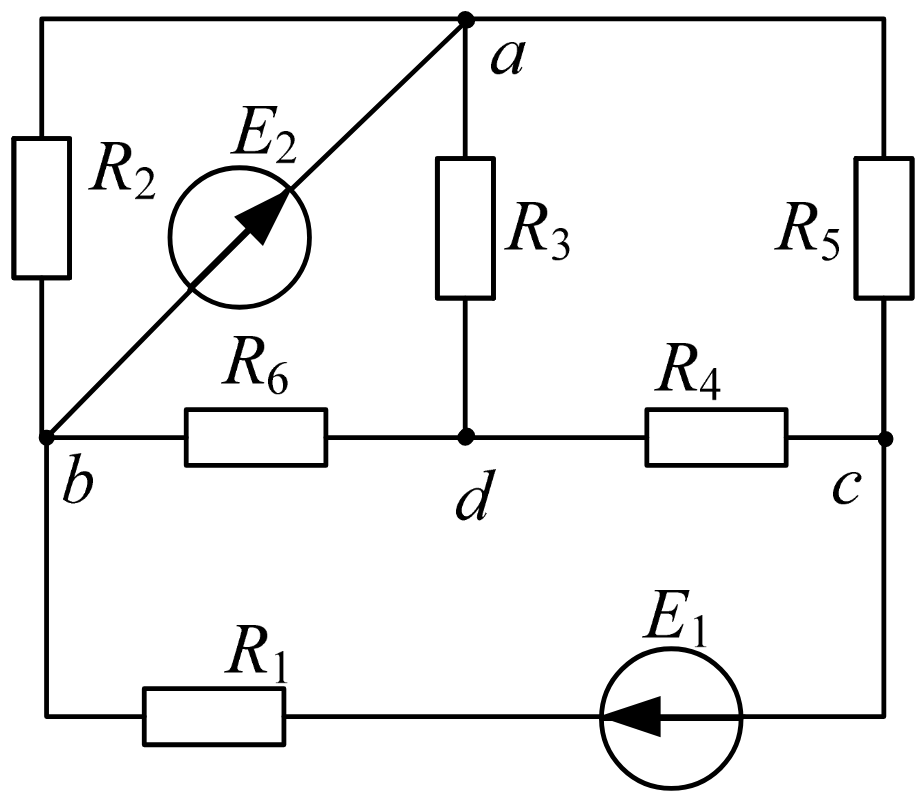
\includegraphics[width=\textwidth]{images/4_task.png}
        \caption{Вариант \#4}
        \label{fig:task_4}
    \end{minipage}
\end{figure}

% Ряд 3: Задачи 5-6
\begin{figure}[H]
    \centering
    \begin{minipage}{0.48\textwidth}
        \centering
        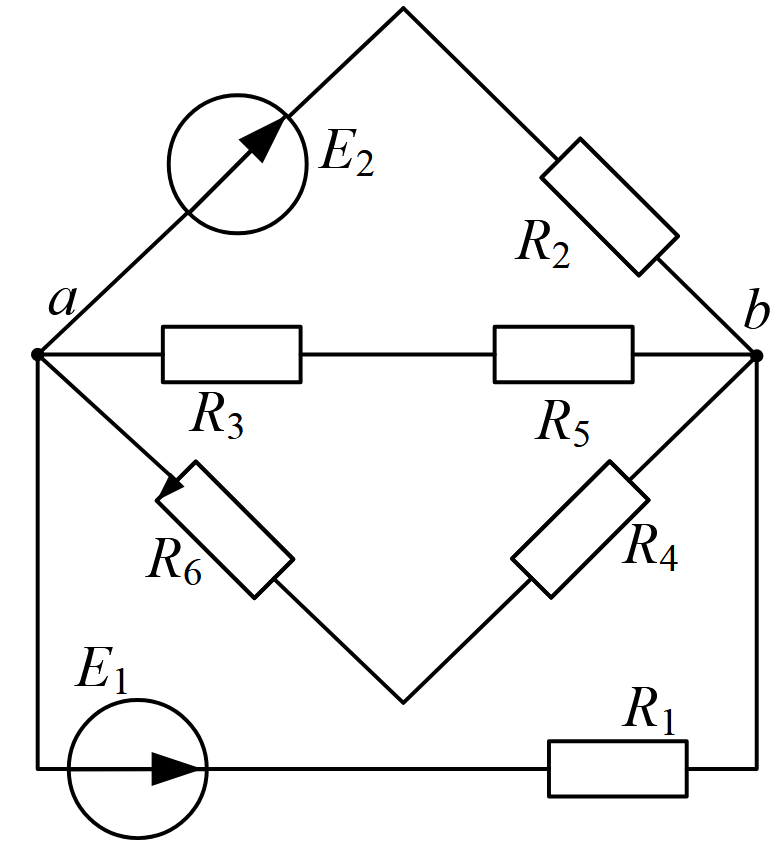
\includegraphics[width=\textwidth]{images/5_task.png}
        \caption{Вариант \#5}
        \label{fig:task_5}
    \end{minipage}
    \hfill
    \begin{minipage}{0.48\textwidth}
        \centering
        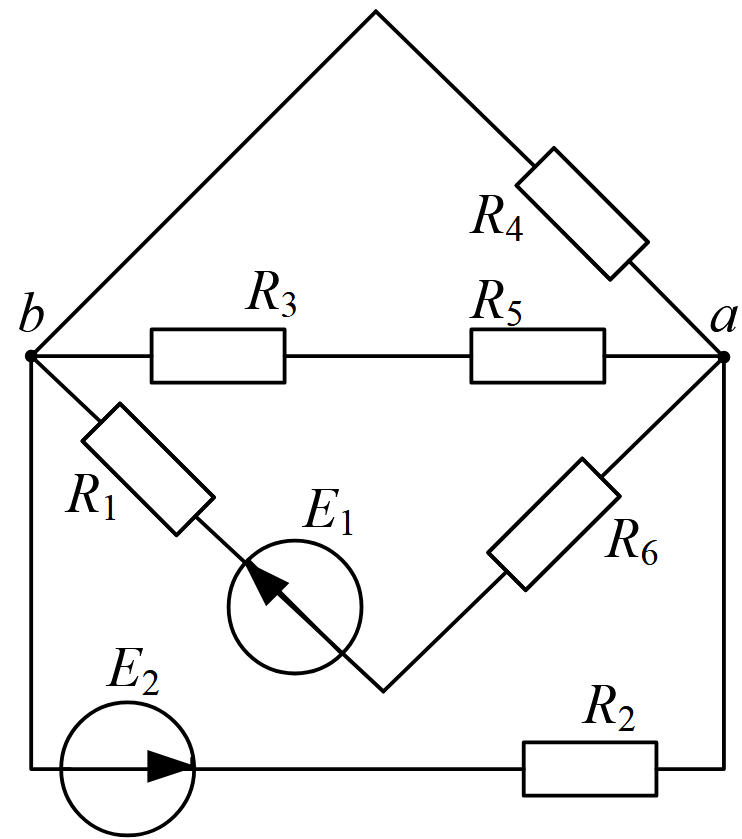
\includegraphics[width=\textwidth]{images/6_task.png}
        \caption{Вариант \#6}
        \label{fig:task_6}
    \end{minipage}
\end{figure}

% Ряд 4: Задачи 7-8
\begin{figure}[H]
    \centering
    \begin{minipage}{0.48\textwidth}
        \centering
        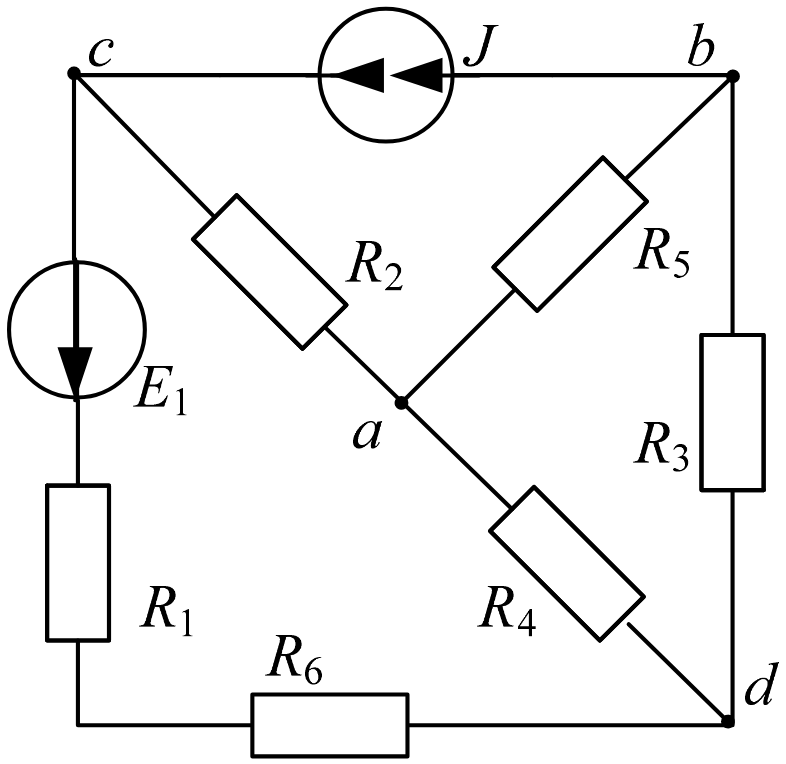
\includegraphics[width=\textwidth]{images/7_task.png}
        \caption{Вариант \#7}
        \label{fig:task_7}
    \end{minipage}
    \hfill
    \begin{minipage}{0.48\textwidth}
        \centering
        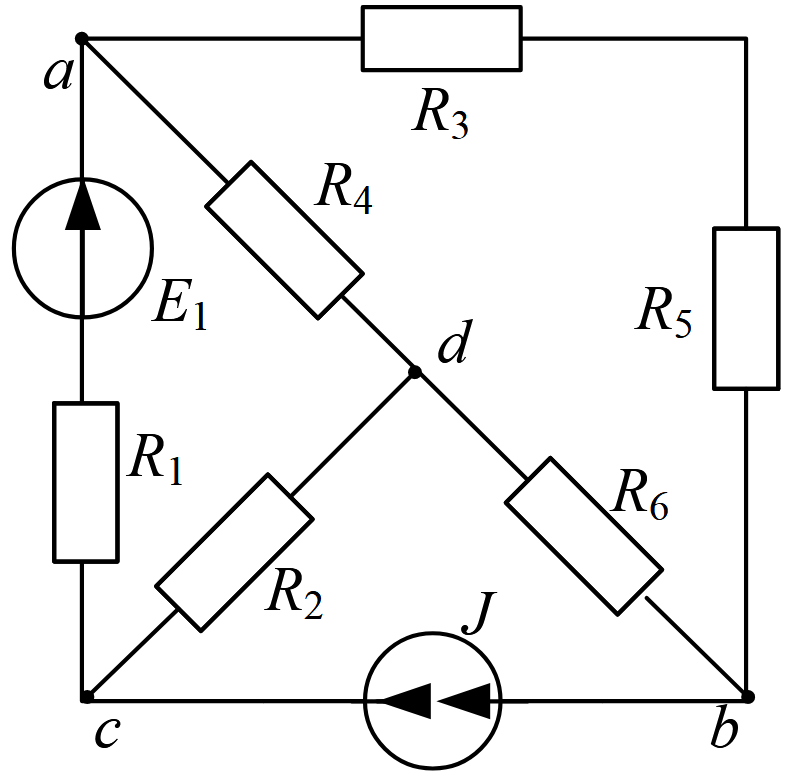
\includegraphics[width=\textwidth]{images/8_task.png}
        \caption{Вариант \#8}
        \label{fig:task_8}
    \end{minipage}
\end{figure}

% Ряд 5: Задачи 9-10
\begin{figure}[H]
    \centering
    \begin{minipage}{0.48\textwidth}
        \centering
        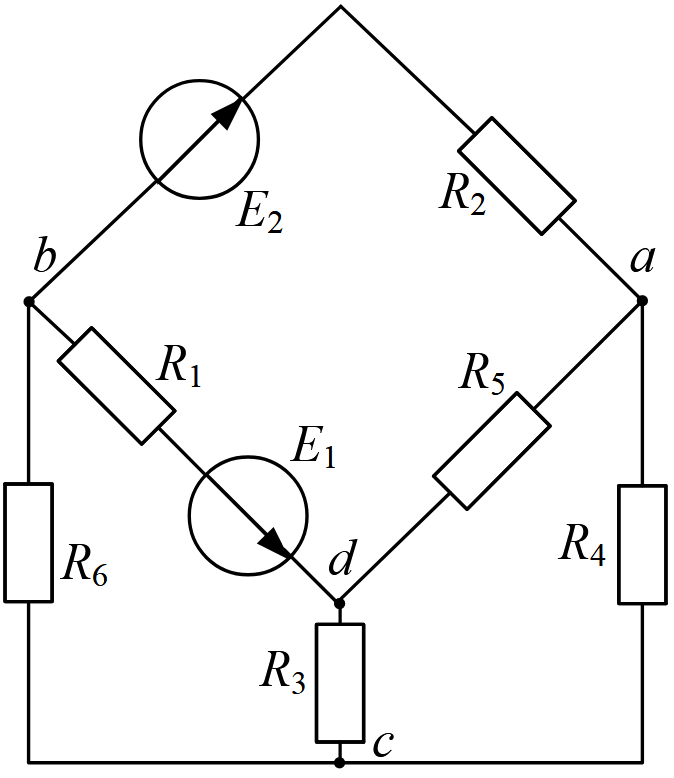
\includegraphics[width=\textwidth]{images/9_task.png}
        \caption{Вариант \#9}
        \label{fig:task_9}
    \end{minipage}
    \hfill
    \begin{minipage}{0.48\textwidth}
        \centering
        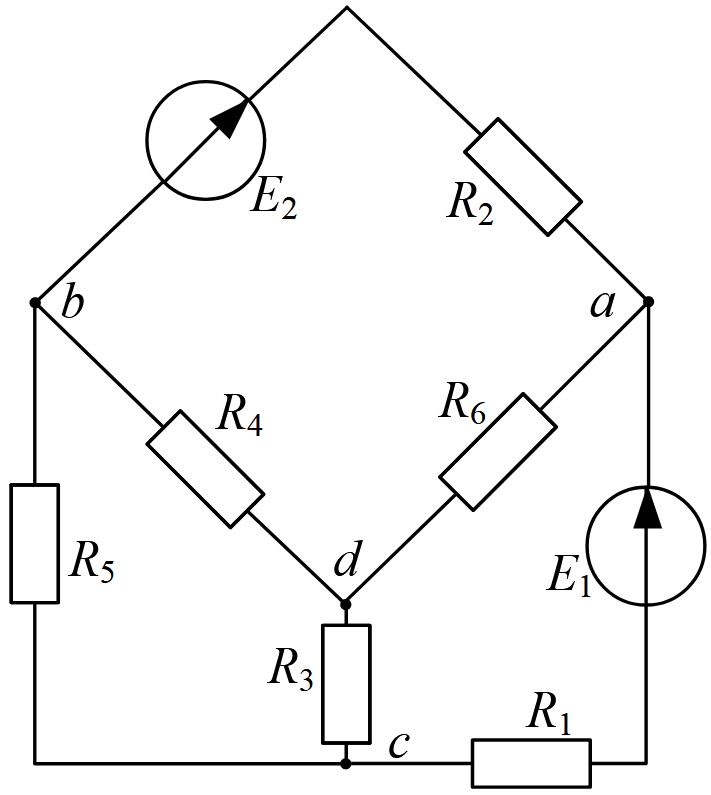
\includegraphics[width=\textwidth]{images/10_task.png}
        \caption{Вариант \#10}
        \label{fig:task_10}
    \end{minipage}
\end{figure}

% Ряд 6: Задачи 11-12
\begin{figure}[H]
    \centering
    \begin{minipage}{0.48\textwidth}
        \centering
        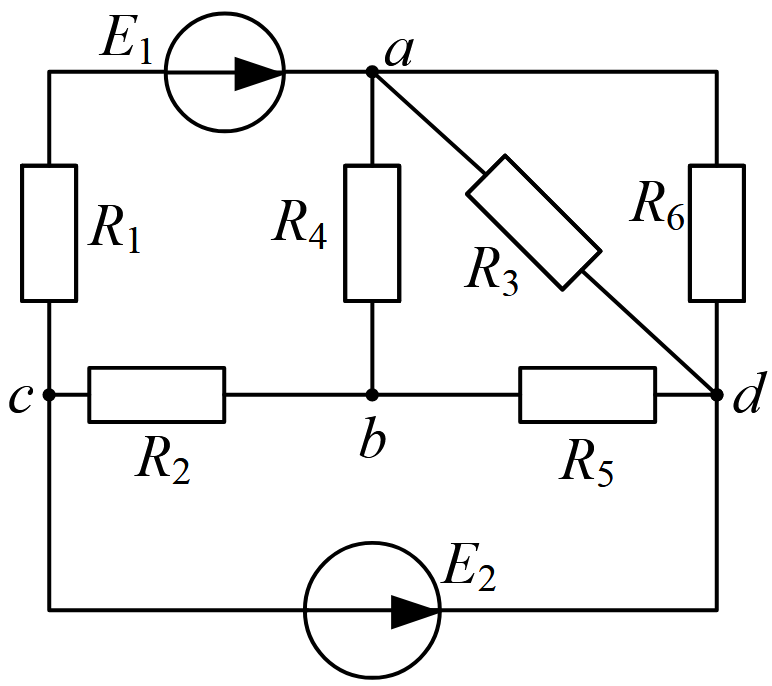
\includegraphics[width=\textwidth]{images/11_task.png}
        \caption{Вариант \#11}
        \label{fig:task_11}
    \end{minipage}
    \hfill
    \begin{minipage}{0.48\textwidth}
        \centering
        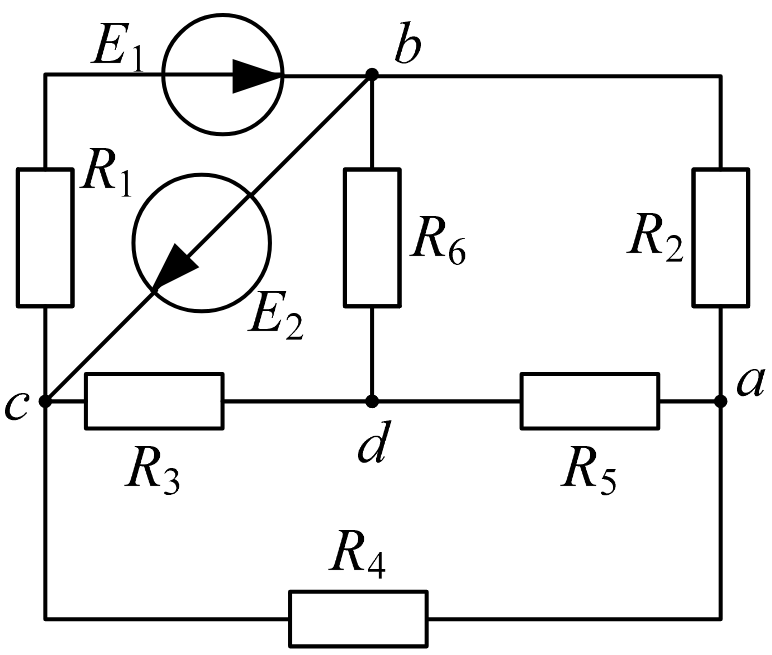
\includegraphics[width=\textwidth]{images/12_task.png}
        \caption{Вариант \#12}
        \label{fig:task_12}
    \end{minipage}
\end{figure}

% Ряд 7: Задачи 13-14
\begin{figure}[H]
    \centering
    \begin{minipage}{0.48\textwidth}
        \centering
        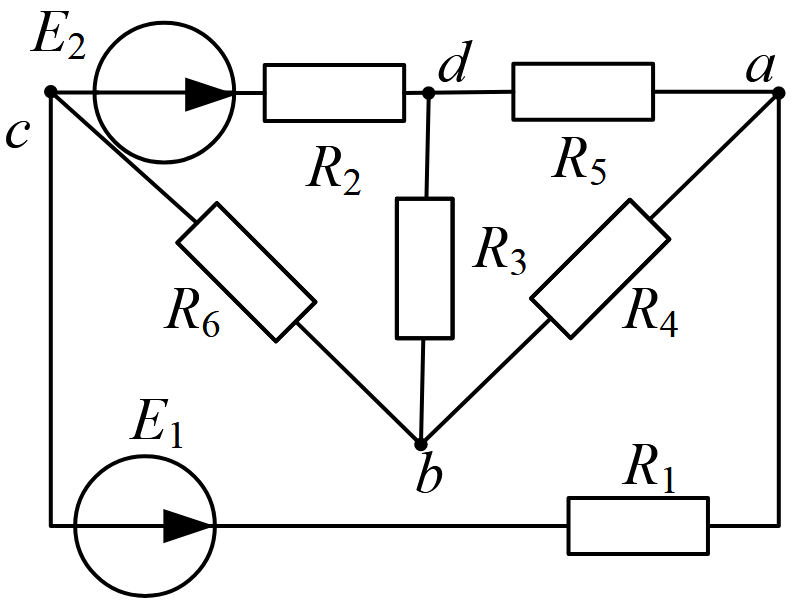
\includegraphics[width=\textwidth]{images/13_task.png}
        \caption{Вариант \#13}
        \label{fig:task_13}
    \end{minipage}
    \hfill
    \begin{minipage}{0.48\textwidth}
        \centering
        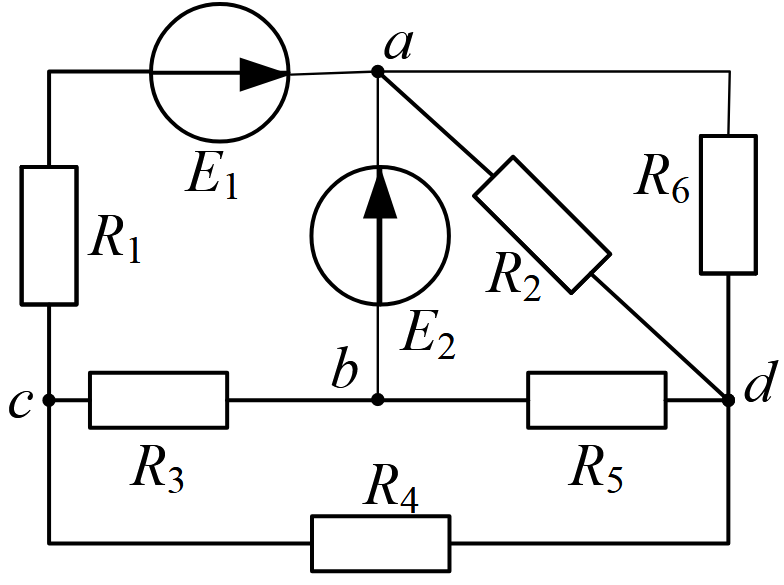
\includegraphics[width=\textwidth]{images/14_task.png}
        \caption{Вариант \#14}
        \label{fig:task_14}
    \end{minipage}
\end{figure}

% Ряд 8: Задачи 15-16
\begin{figure}[H]
    \centering
    \begin{minipage}{0.48\textwidth}
        \centering
        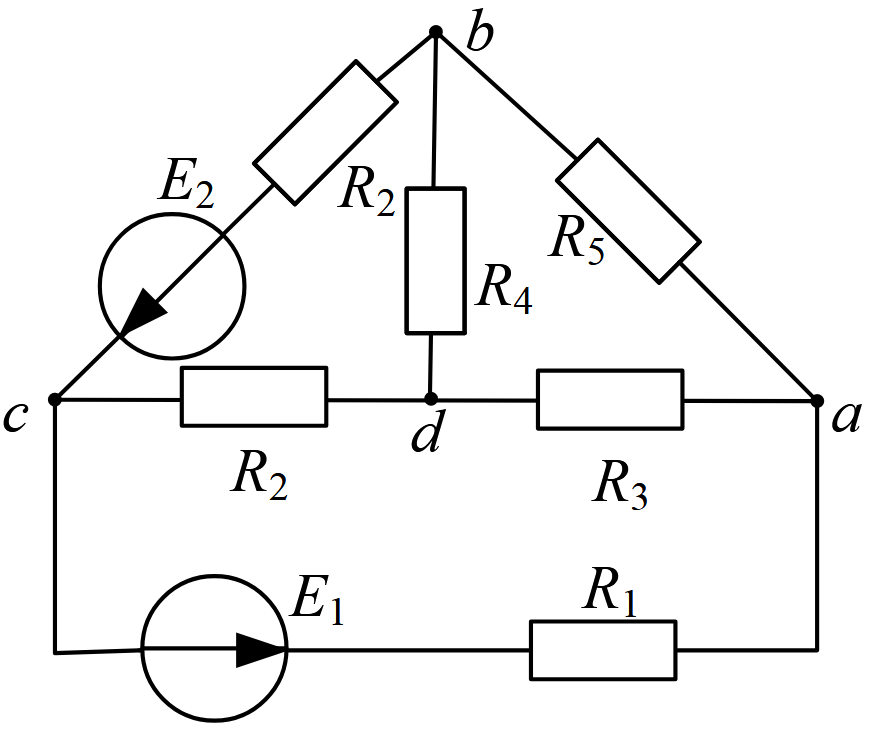
\includegraphics[width=\textwidth]{images/15_task.png}
        \caption{Вариант \#15}
        \label{fig:task_15}
    \end{minipage}
    \hfill
    \begin{minipage}{0.48\textwidth}
        \centering
        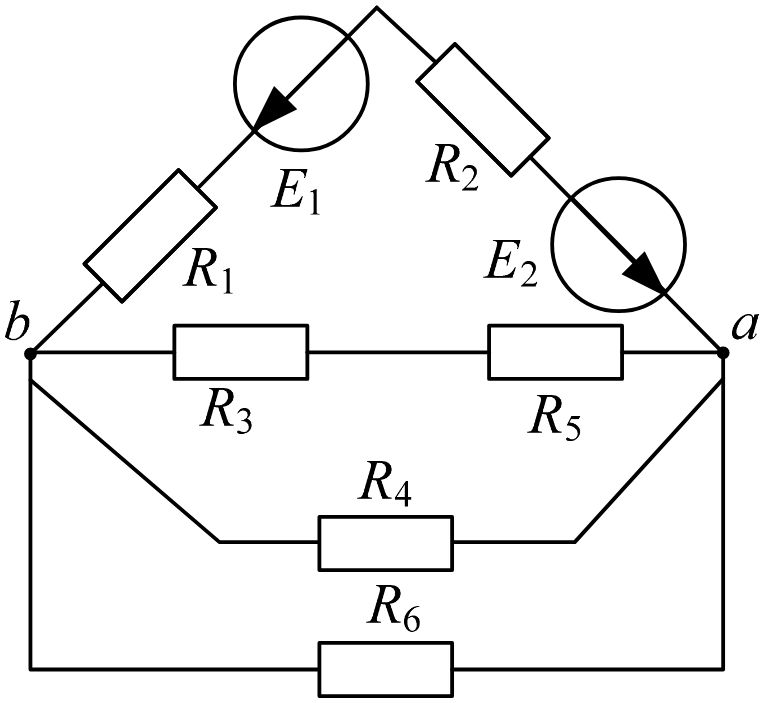
\includegraphics[width=\textwidth]{images/16_task.png}
        \caption{Вариант \#16}
        \label{fig:task_16}
    \end{minipage}
\end{figure}

% Ряд 9: Задачи 17-18
\begin{figure}[H]
    \centering
    \begin{minipage}{0.48\textwidth}
        \centering
        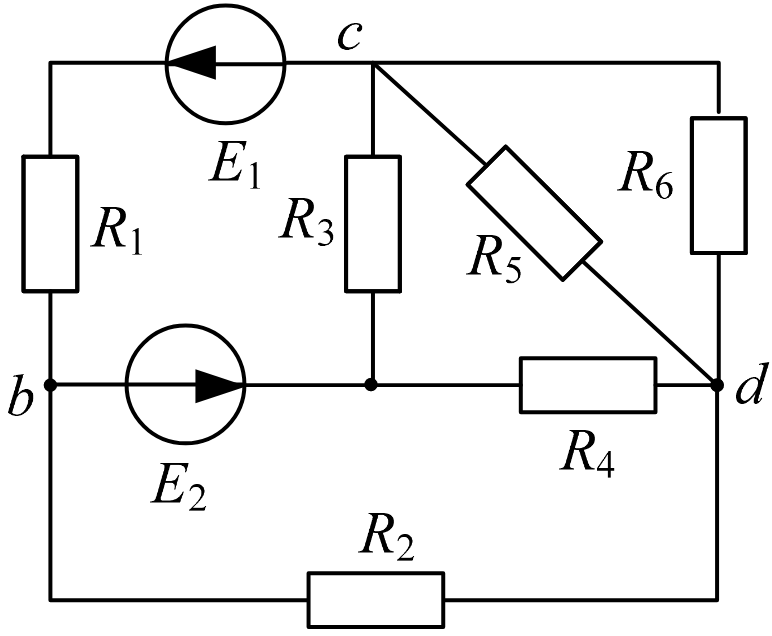
\includegraphics[width=\textwidth]{images/17_task.png}
        \caption{Вариант \#17}
        \label{fig:task_17}
    \end{minipage}
    \hfill
    \begin{minipage}{0.48\textwidth}
        \centering
        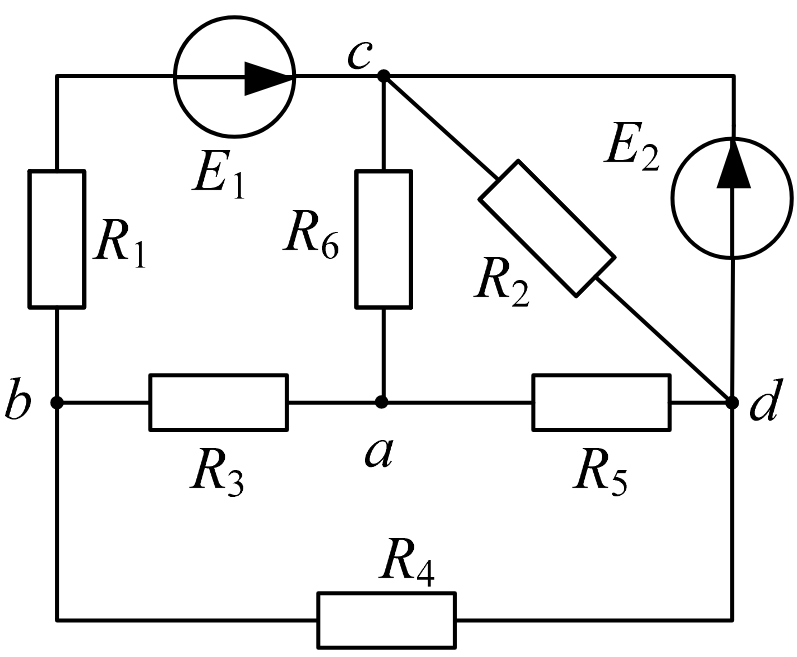
\includegraphics[width=\textwidth]{images/18_task.png}
        \caption{Вариант \#18}
        \label{fig:task_18}
    \end{minipage}
\end{figure}

% Ряд 10: Задачи 19-20
\begin{figure}[H]
    \centering
    \begin{minipage}{0.48\textwidth}
        \centering
        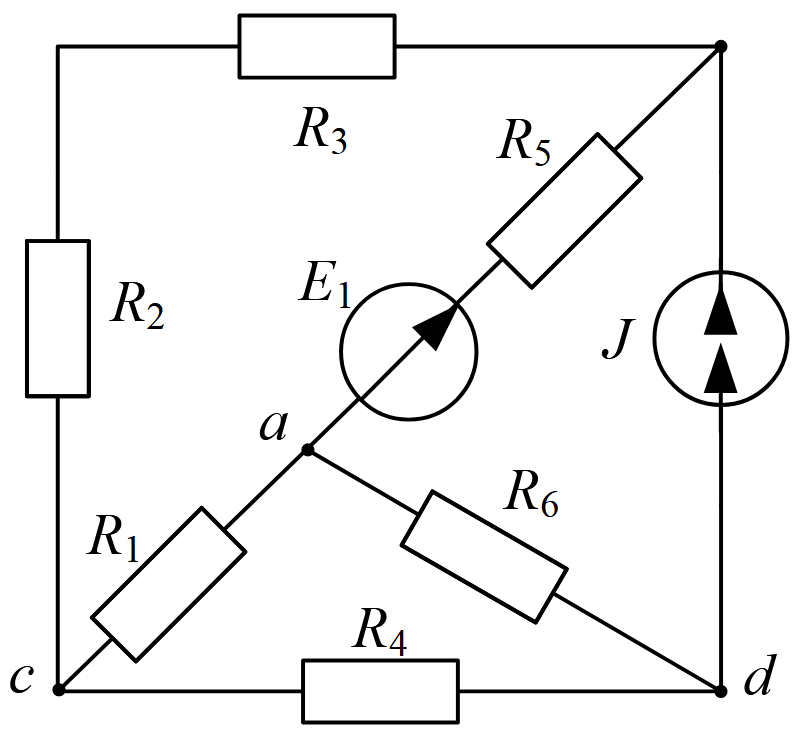
\includegraphics[width=\textwidth]{images/19_task.png}
        \caption{Вариант \#19}
        \label{fig:task_19}
    \end{minipage}
    \hfill
    \begin{minipage}{0.48\textwidth}
        \centering
        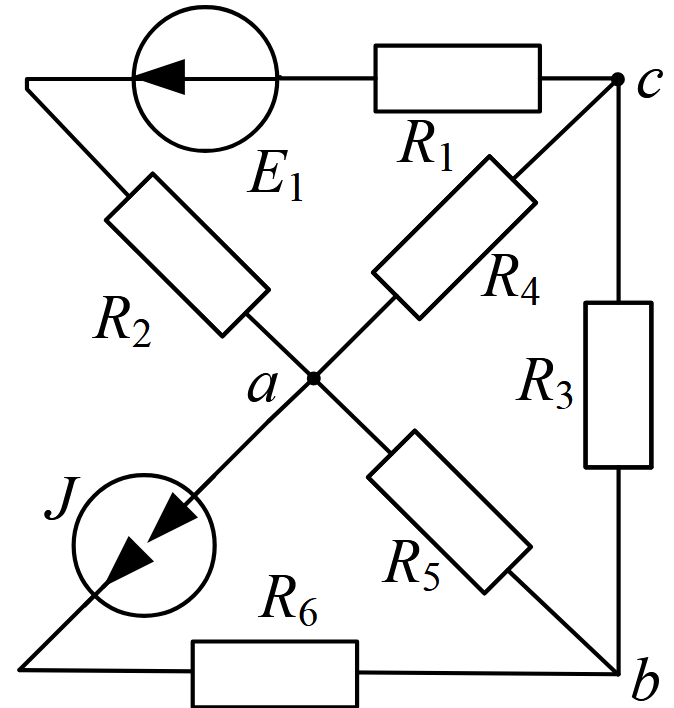
\includegraphics[width=\textwidth]{images/20_task.png}
        \caption{Вариант \#20}
        \label{fig:task_20}
    \end{minipage}
\end{figure}

% Ряд 11: Задачи 21-22
\begin{figure}[H]
    \centering
    \begin{minipage}{0.48\textwidth}
        \centering
        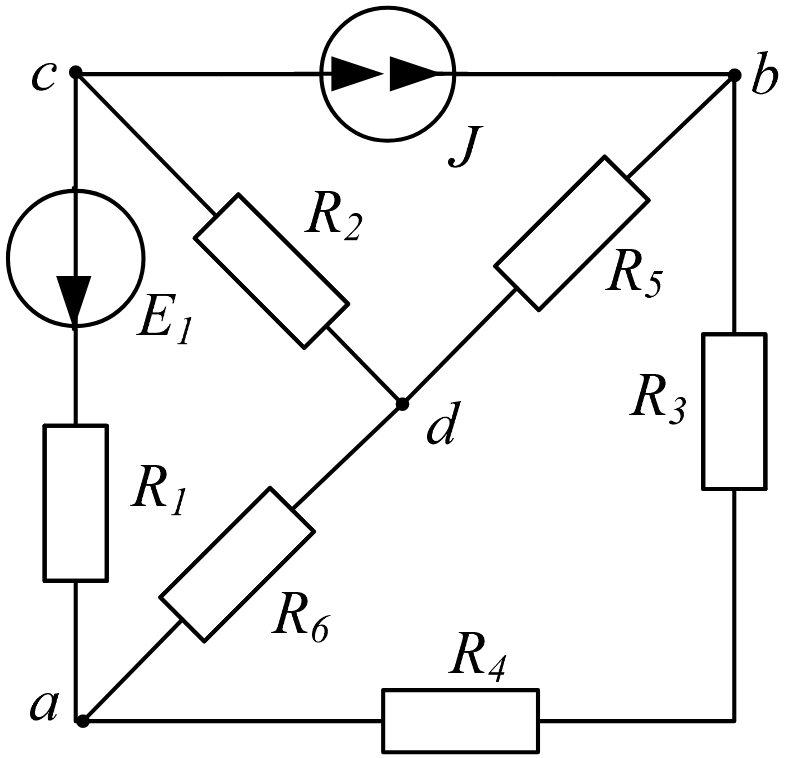
\includegraphics[width=\textwidth]{images/21_task.png}
        \caption{Вариант \#21}
        \label{fig:task_21}
    \end{minipage}
    \hfill
    \begin{minipage}{0.48\textwidth}
        \centering
        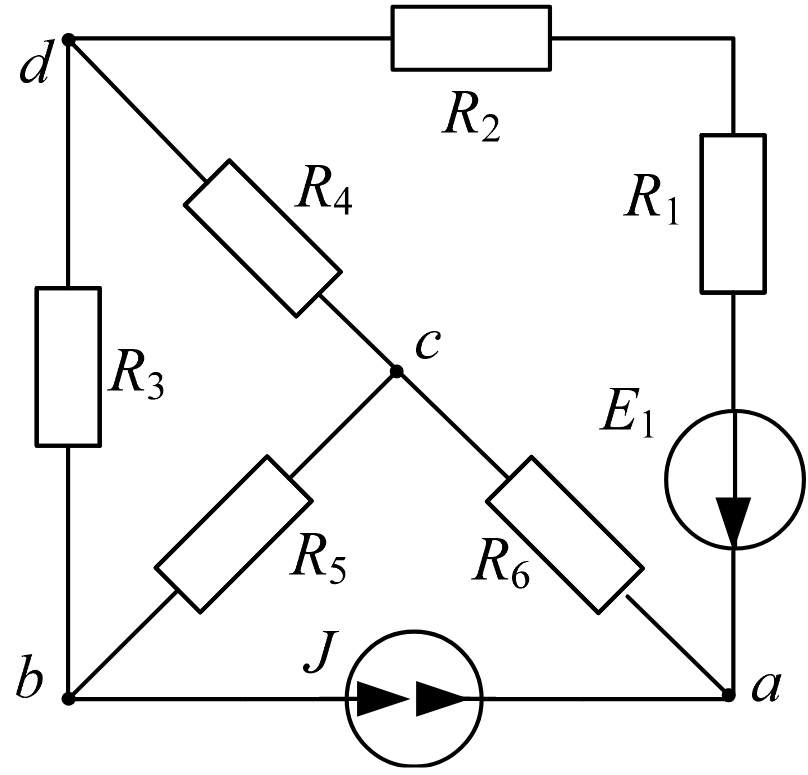
\includegraphics[width=\textwidth]{images/22_task.png}
        \caption{Вариант \#22}
        \label{fig:task_22}
    \end{minipage}
\end{figure}

% Ряд 12: Задачи 23-24
\begin{figure}[H]
    \centering
    \begin{minipage}{0.48\textwidth}
        \centering
        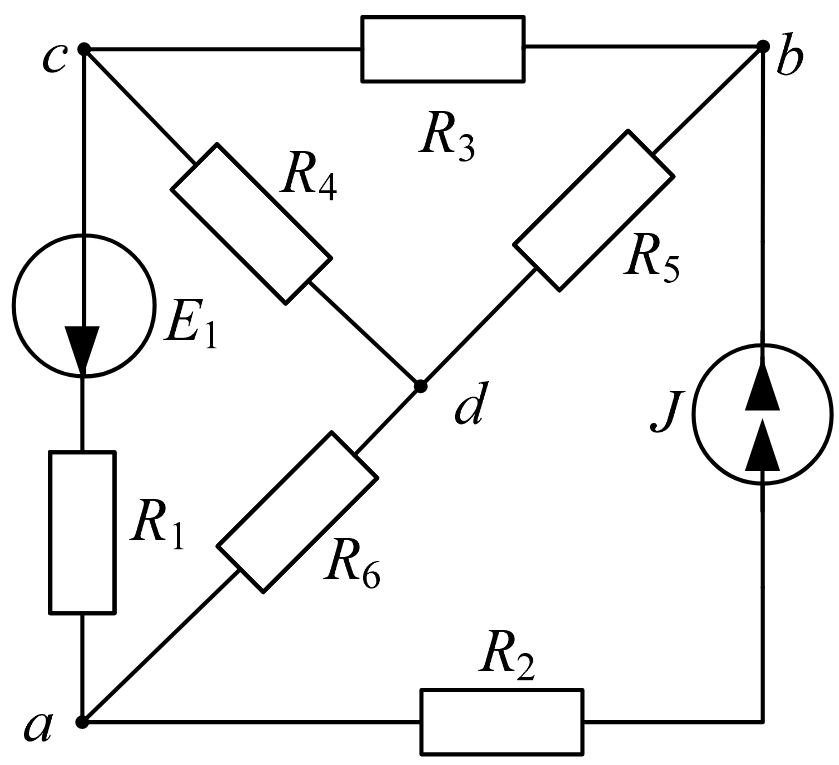
\includegraphics[width=\textwidth]{images/23_task.png}
        \caption{Вариант \#23}
        \label{fig:task_23}
    \end{minipage}
    \hfill
    \begin{minipage}{0.48\textwidth}
        \centering
        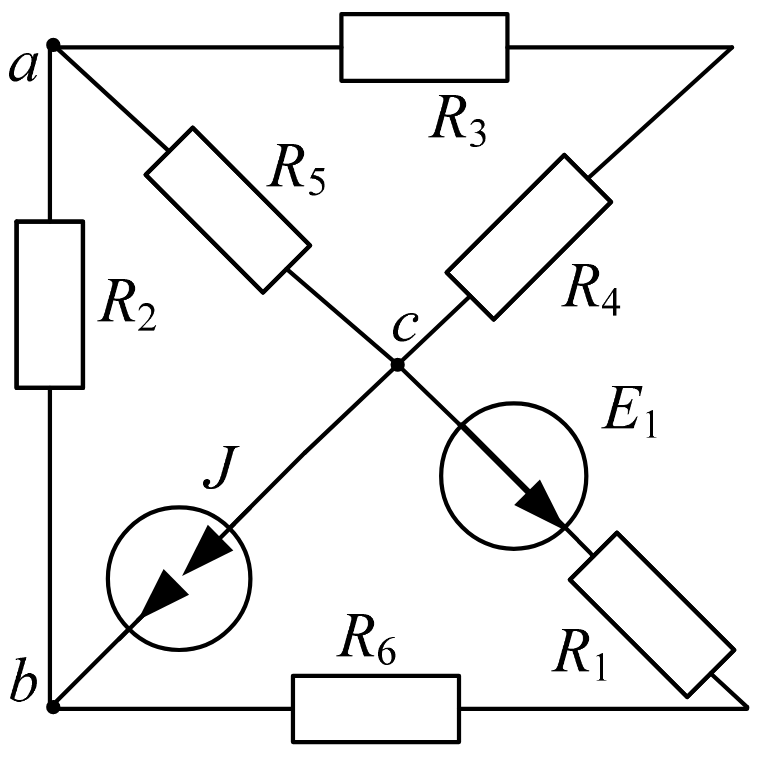
\includegraphics[width=\textwidth]{images/24_task.png}
        \caption{Вариант \#24}
        \label{fig:task_24}
    \end{minipage}
\end{figure}

% Ряд 13: Задачи 25-26
\begin{figure}[H]
    \centering
    \begin{minipage}{0.48\textwidth}
        \centering
        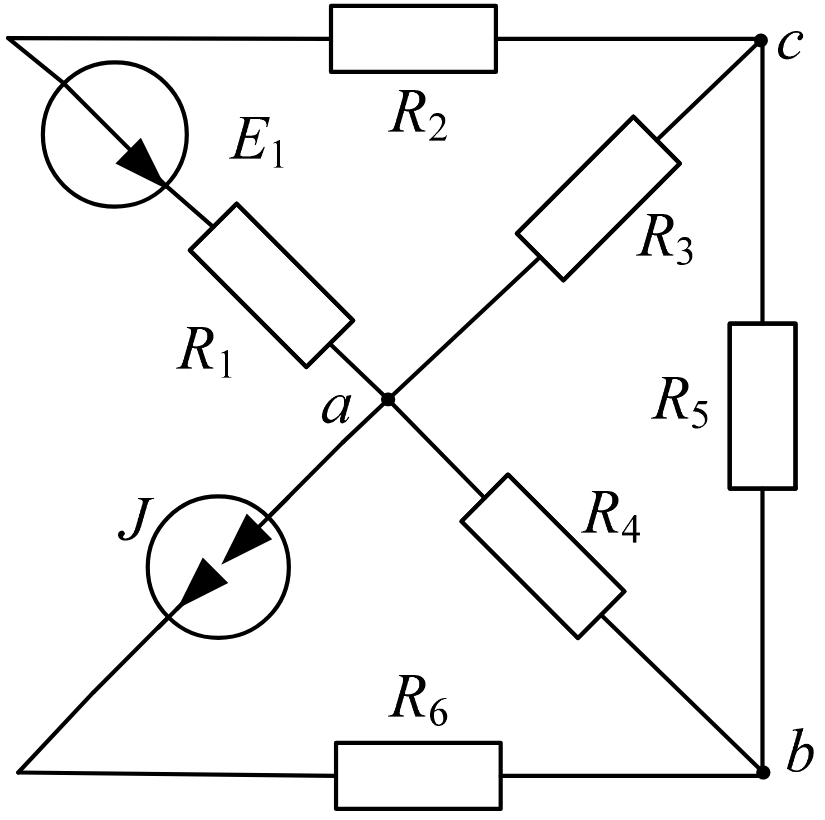
\includegraphics[width=\textwidth]{images/25_task.png}
        \caption{Вариант \#25}
        \label{fig:task_25}
    \end{minipage}
    \hfill
    \begin{minipage}{0.48\textwidth}
        \centering
        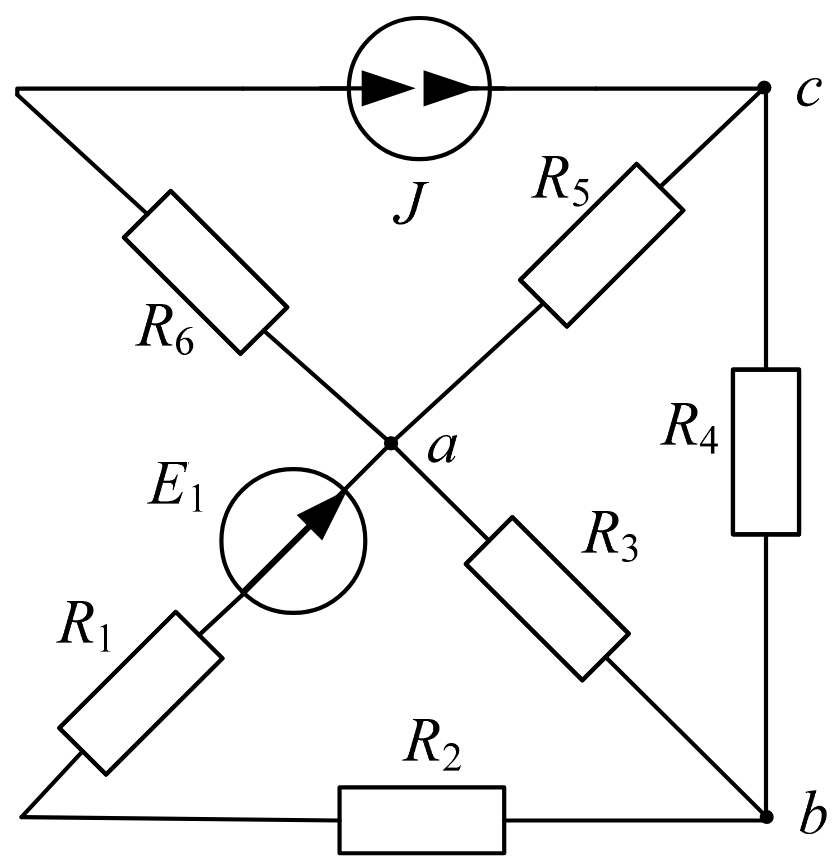
\includegraphics[width=\textwidth]{images/26_task.png}
        \caption{Вариант \#26}
        \label{fig:task_26}
    \end{minipage}
\end{figure}

% Ряд 14: Задачи 27-28
\begin{figure}[H]
    \centering
    \begin{minipage}{0.48\textwidth}
        \centering
        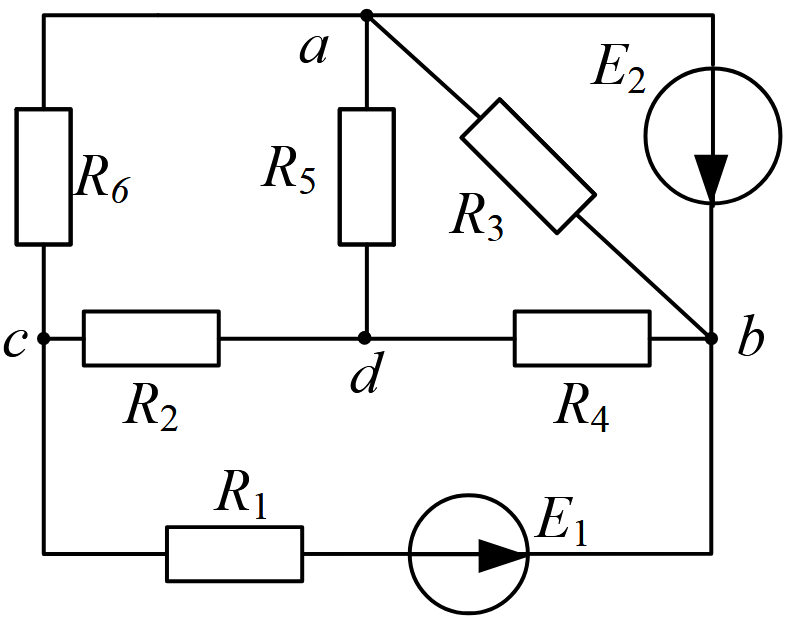
\includegraphics[width=\textwidth]{images/27_task.png}
        \caption{Вариант \#27}
        \label{fig:task_27}
    \end{minipage}
    \hfill
    \begin{minipage}{0.48\textwidth}
        \centering
        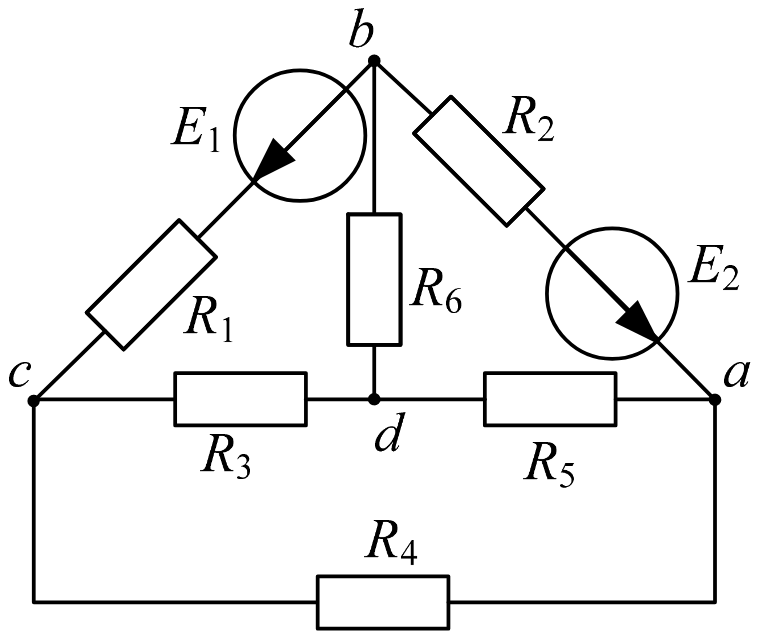
\includegraphics[width=\textwidth]{images/28_task.png}
        \caption{Вариант \#28}
        \label{fig:task_28}
    \end{minipage}
\end{figure}
